% !TeX spellcheck = en_EN-English
\documentclass[a4paper]{article}
\usepackage[slovak]{babel}
\usepackage[utf8]{inputenc}
\usepackage[T1]{fontenc}
\usepackage{a4wide}
\usepackage{amsmath}
\usepackage{amsfonts}
\usepackage{amssymb}
\usepackage{mathrsfs}
\usepackage[small,bf]{caption}
\usepackage{subcaption}
\usepackage{xcolor}
\usepackage{graphicx}
\usepackage{enumerate}
\usepackage{hyperref}



\pagestyle{empty}
\setlength{\parindent}{0pt}

\newenvironment{modenumerate}
{\enumerate\setupmodenumerate}
{\endenumerate}

\newif\ifmoditem
\newcommand{\setupmodenumerate}{%
	\global\moditemfalse
	\let\origmakelabel\makelabel
	\def\moditem##1{\global\moditemtrue\def\mesymbol{##1}\item}%
	\def\makelabel##1{%
		\origmakelabel{##1\ifmoditem\rlap{\mesymbol}\fi\enspace}%
		\global\moditemfalse}%
}

\makeatletter
\def\@seccntformat#1{%
	\expandafter\ifx\csname c@#1\endcsname\c@section\else
	\csname the#1\endcsname\quad
	\fi}
\makeatother

\begin{document} 
	
	\pagenumbering{arabic}
	\pagestyle{plain}
	
	\begin{center}
		\sc\large
		ML Homework 5
		
	\end{center}
	Autor: Marián Kravec
	(Prosím Vlado nestrácaj s kontrolou tohto veľa času, nevedel som čo k tomu chcem napísať, ale keď už som vygeneroval grafy tak som sa rozhodol to odovzdať)
	\\
	\\
	\\
	We will create dataset using provided function that create data with XOR pattern, however we add more functionality to generative function. We add possibility to set noise coefficient (fraction of samples that would be incorrectly labeled) and to set center of decision boundary.
	
	We will create 3 training datasets. First will have 1000 samples (will be biggest) with small noise (only 1\%) and decision boundary will stay in middle. It can be considered as desired dataset (big, with little noise). Second will opposite of the first with only 100 samples and high noise (25\%), it will also have moved decision boundary higher (it will split  y-axis into 1/4 and 3/4 instead of 1/2 and 1/2). Third dataset will be something in-between from size and noise values with 300 samples and 10\% noise, however  decision boundary will be moved closer to top right corner and will split both axis into 1/4 and 3/4.
	
	For each of these datasets we prepare validation dataset with 100 samples and same values noise and  decision boundary as respective training set. 
	\\
	\\
	Let's start with first dataset. Firstly let's take a look at how SVD compute boundaries for combination of 3 values of $C$ (0.1, 1, 10) and 3 values of $\gamma$ (0.1, 1, 10):
	
	\centerline{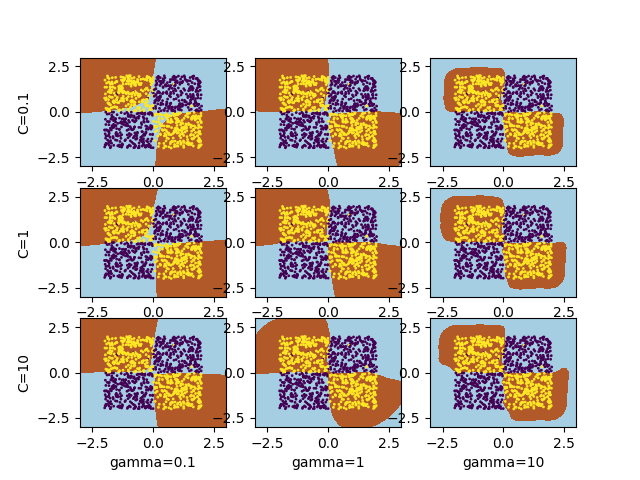
\includegraphics[width=1.1\textwidth]{dataset_1_diff_c_gamma}}
	
	Now let's plot scores of prediction for different values of $C$ and $\gamma$ for both training and validation dataset (plots with different $C$ values have $\gamma=1$ and plots with different $\gamma$ values have $C=1$):
	
	\centerline{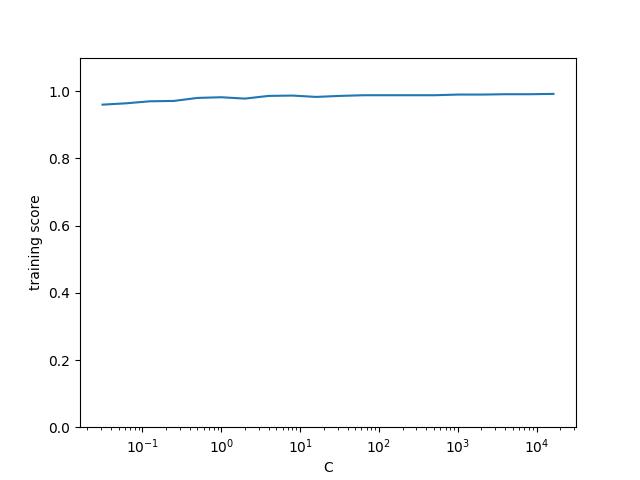
\includegraphics[width=1\textwidth]{dataset_1_train_C_scores}}  
	
	\centerline{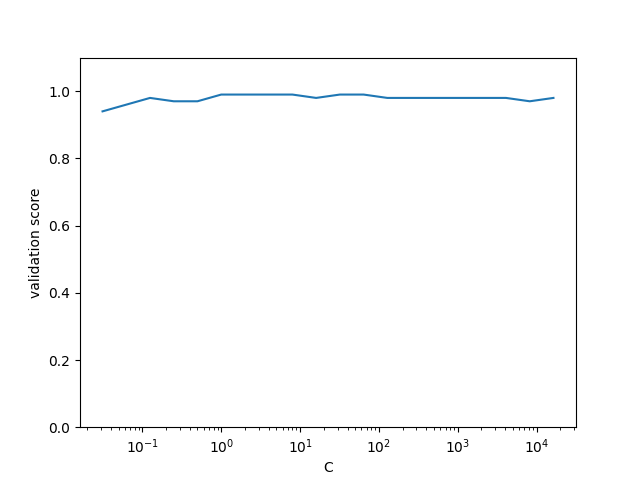
\includegraphics[width=1\textwidth]{dataset_1_validation_C_scores}}  
	
	\centerline{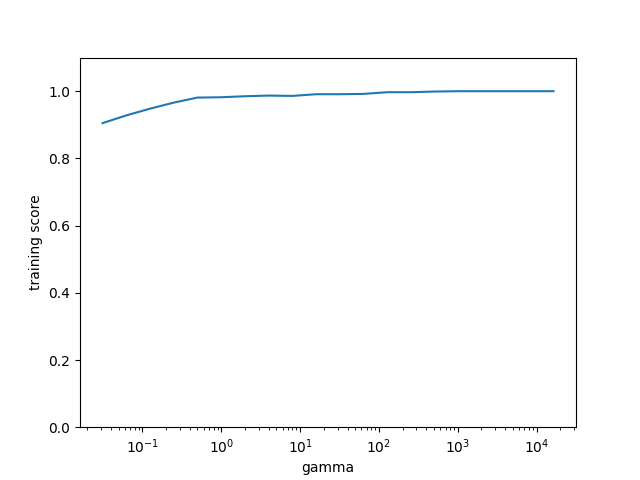
\includegraphics[width=1\textwidth]{dataset_1_train_gamma_scores}}  
	
	\centerline{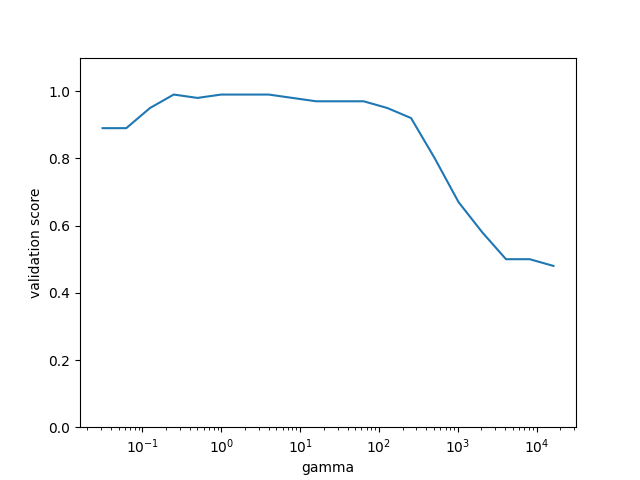
\includegraphics[width=1\textwidth]{dataset_1_validation_gamma_scores}}  
	
	In both cases (both $C$ and $\gamma$) we can see that as values of hyperparameter increase training score get closer to 1 (perfect score). How ever in case of validation score we can see that in case of $C$ hyperparameter this score fluctuate close to 1 for all values but in case of $\gamma$ hyperparameter validation score at first increase (it's lower for very small values) then it fluctuate close to 1 but then it suddenly start dropping which mostly likely mean that those models are overfitted.
	
	As a final plot let's take a look at heatmaps for different values of $C$ and $\gamma$ for both training and validation data:
	
	\centerline{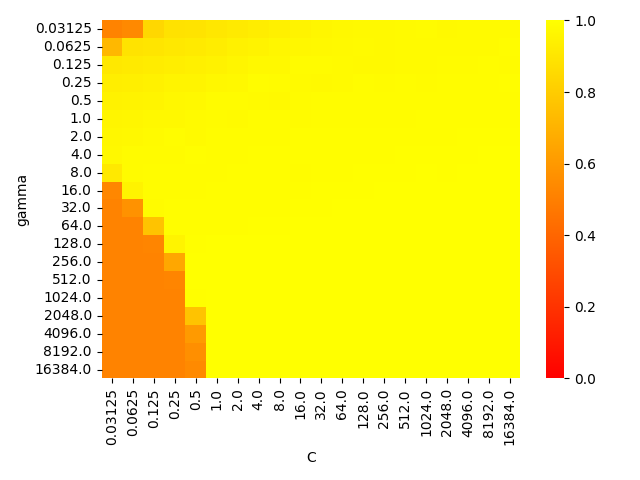
\includegraphics[width=0.7\textwidth]{dataset_1_train_heatmap_scores}}  
	
	\centerline{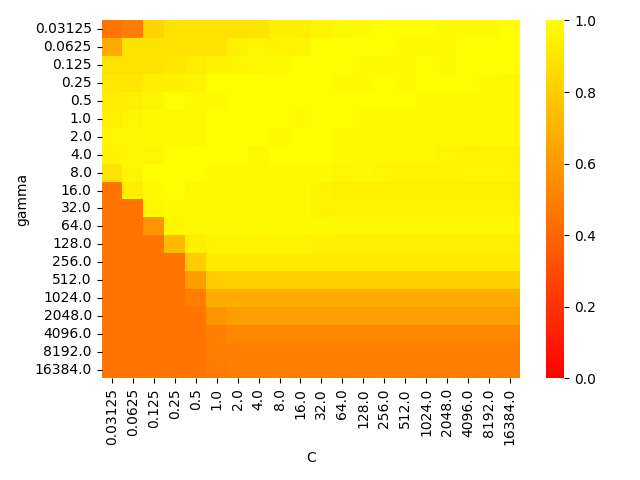
\includegraphics[width=0.7\textwidth]{dataset_1_validation_heatmap_scores}}  
	
	We can see similar behavior as in lineplots however we also see that for small values $C$ and large values of $\gamma$ we get decreasing even training score.
	\newpage
	Now let's move to second dataset (we will create same plots).
	
	\centerline{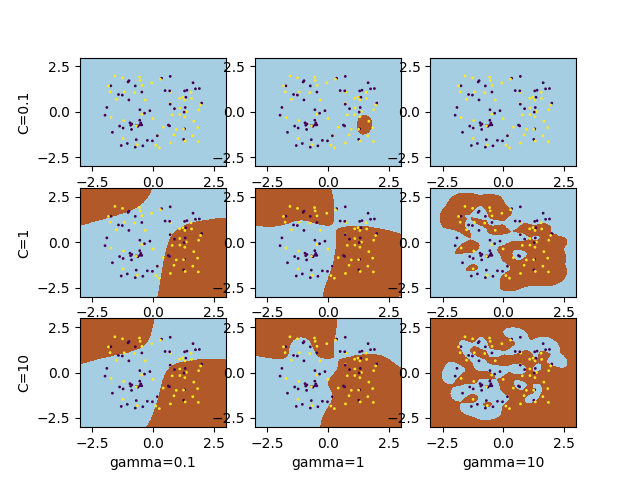
\includegraphics[width=1.1\textwidth]{dataset_2_diff_c_gamma}}
	
	In this case we can see that small values of $C$ have hard time identifying any yellow point in such noisy dataset. We can also see opposite extreme where for large values of both hyperparameters it tries to identify all points perfectly which leads to overfitting.  
	
	\centerline{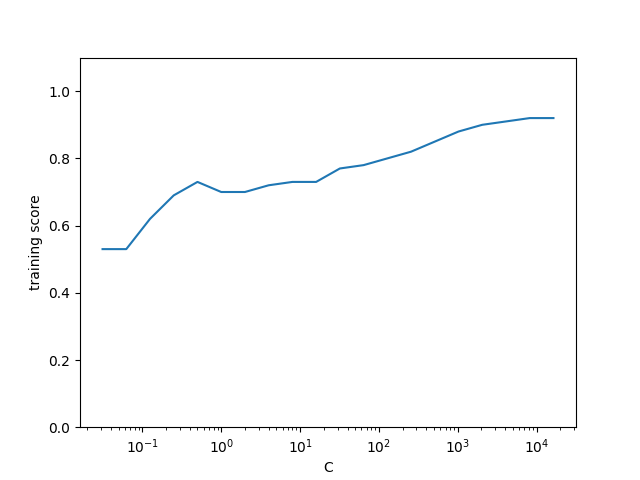
\includegraphics[width=1\textwidth]{dataset_2_train_C_scores}}  
	
	\centerline{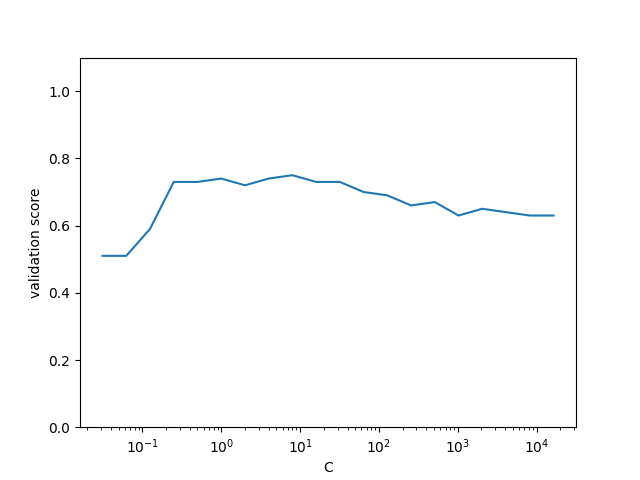
\includegraphics[width=1\textwidth]{dataset_2_validation_C_scores}}  
	
	\centerline{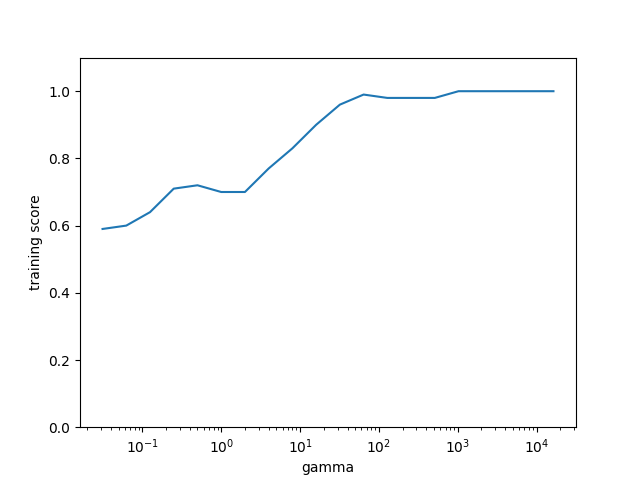
\includegraphics[width=1\textwidth]{dataset_2_train_gamma_scores}}  
	
	\centerline{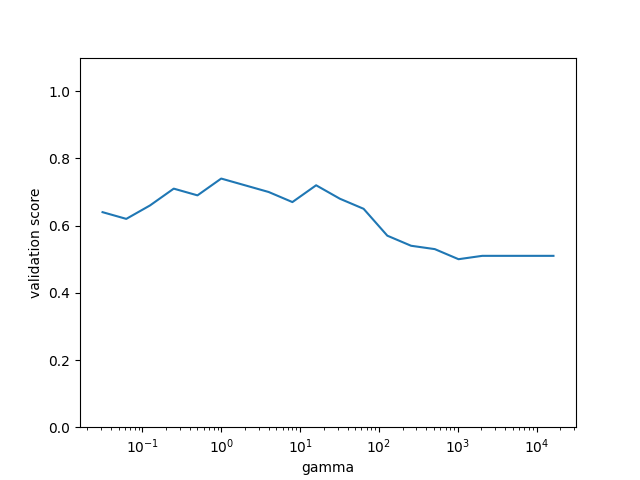
\includegraphics[width=1\textwidth]{dataset_2_validation_gamma_scores}}  
	
	In lineplots we can almost perfectly same behavior as in first dataset (with only different that because of noise validation score is fluctuating around lower numbers)
	
	\centerline{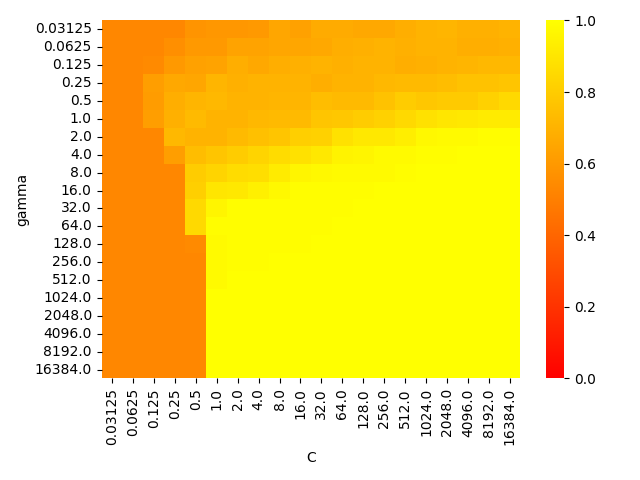
\includegraphics[width=0.7\textwidth]{dataset_2_train_heatmap_scores}}  
	
	\centerline{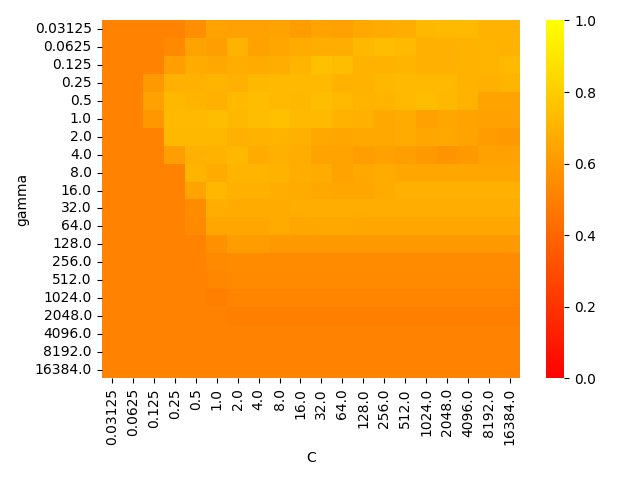
\includegraphics[width=0.7\textwidth]{dataset_2_validation_heatmap_scores}}
	
	\newpage
	Now we take a look at third dataset:
	
	\centerline{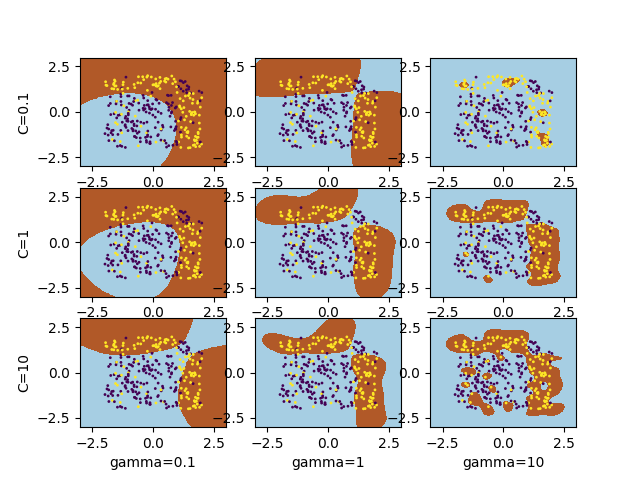
\includegraphics[width=1.1\textwidth]{dataset_3_diff_c_gamma}}
	
	Here is similar behavior to second with only difference that small values of $C$ can identify yellow at least to some extend (at least for smaller values of $\gamma$) most likely thanks to lower noise.   
	
	\centerline{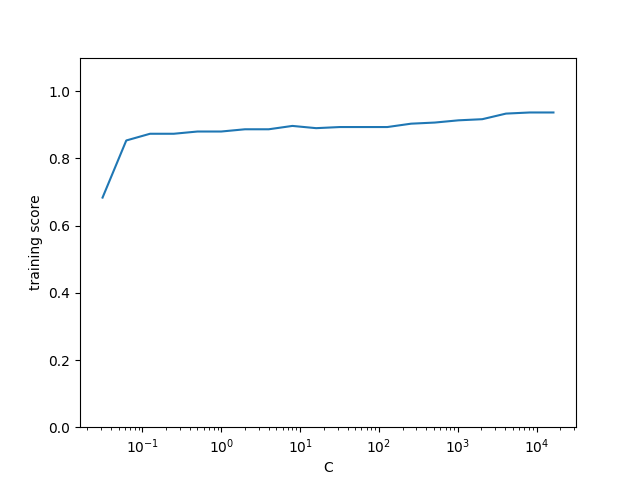
\includegraphics[width=1\textwidth]{dataset_3_train_C_scores}}  
	
	\centerline{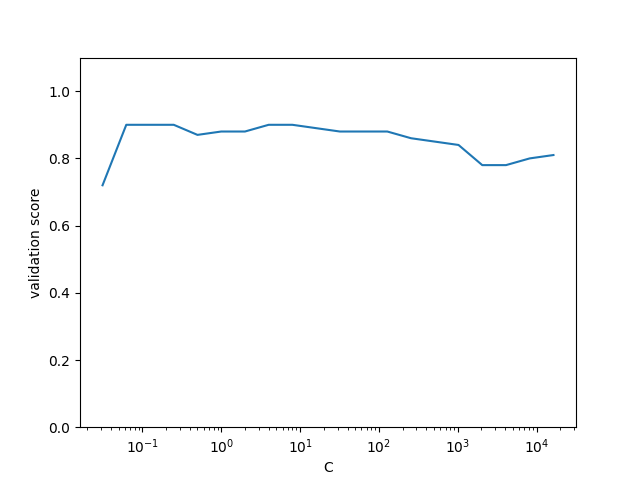
\includegraphics[width=1\textwidth]{dataset_3_validation_C_scores}}  
	
	\centerline{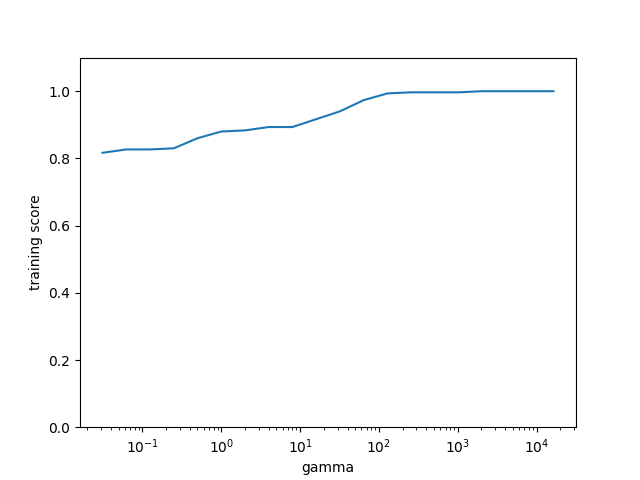
\includegraphics[width=1\textwidth]{dataset_3_train_gamma_scores}}  
	
	\centerline{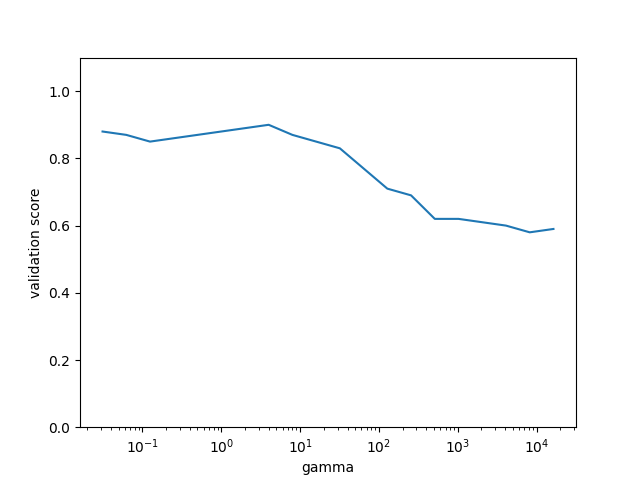
\includegraphics[width=1\textwidth]{dataset_3_validation_gamma_scores}}  
	
	Lineplots are more or same as in previous datasets.
	
	\centerline{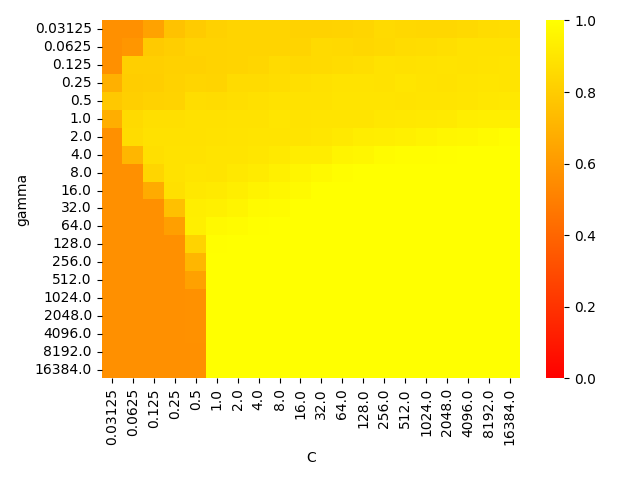
\includegraphics[width=0.7\textwidth]{dataset_3_train_heatmap_scores}}  
	
	\centerline{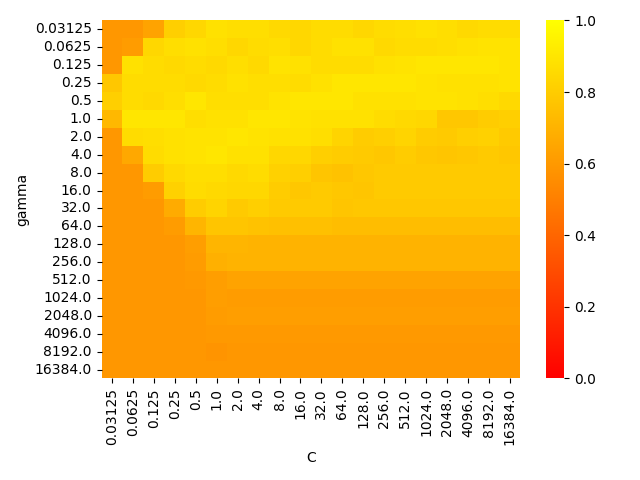
\includegraphics[width=0.7\textwidth]{dataset_3_validation_heatmap_scores}}  
	
	
	All in all we can say that we both hyperparameters behave similarly in a way that as they increase model is trying to fit training data more precisely. Hyperparameter $\gamma$ seems to bigger influence than $C$.
	  
\end{document}